\section{Электричество}

\subsection{Основы электростатики}

\subsubsection{Опыт Милликена}

После открытия электрона встал вопрос об измерении его свойств. Точное измерение заряда электрона --- заслуга Роберта Милликена.

Экспериментальная установка представляла собой плоский конденсатор, в камеру которого распылялись капли масла. Масло использовалось из-за низкой скорости испарения:

\begin{center}
\begin{tikzpicture}[scale=1.2]
    % Пластины конденсатора (делаем их очень жирными для акцента)
    \draw[line width=1.5pt] (0,2) -- (4,2) node[right] {\textbf{+}};
    \draw[line width=1.5pt] (0,0) -- (4,0) node[right] {\textbf{--}};
    
    % Источник напряжения (батарея)
    \draw (0,2) -- (-1,2) -- (-1,1.1);
    \draw (0,0) -- (-1,0) -- (-1,0.9);
    \draw[line width=1.2pt] (-1.3,1.1) -- (-0.7,1.1); % Положительный полюс
    \draw[line width=1.2pt] (-1.1,0.9) -- (-0.9,0.9); % Отрицательный полюс
    \node at (-1.5,1) {$U$};
    
    % Векторы сил (используем разную толщину и наконечники стрелок для различия)
    % Электрическая сила (вверх) - сделаем ее полой стрелкой или просто жирной
    \draw[-{Stealth[scale=1.2]}, line width=1.4pt] (2,1.1) -- (2,1.9) node[left] {$\vec{F}_{E}$};
    
    % Сила тяжести (вниз) - сделаем ее двойной линией
    \draw[-{Stealth[scale=1.2]}, double, double distance=1pt, thick] (2,1.1) -- (2,0.3) node[left] {$m\vec{g}$};

    % Масляная капля (используем серую заливку или просто черный круг)
    \filldraw[fill=gray!40, draw=black, thick] (2,1.1) circle (2.8pt) node[right=4pt, black] {$q$};
    
    % Линии поля (тонкий пунктир)
    \foreach \x in {0.5, 1.5, 2.5, 3.5}
        \draw[->, dash dot, thin, black!60] (\x,1.8) -- (\x,0.2);
    \node[black!60] at (3.8, 1) {$\vec{E}$};
    
    % Опционально: рамка камеры (тонкая линия)
    \draw[thin, dashed, gray] (-0.2,-0.2) rectangle (4.2,2.2);
\end{tikzpicture}
\end{center}

Сначала рассматривается свободное падение капли при выключенном электрическом поле. Капля движется с установившейся скоростью $v_0$.
Запишем второй закон Ньютона в проекции на вертикальную ось:
\[
F_{\text{тяж}} = F_{\text{арх}} + F_{\text{сопр}}
\]
Раскроем силы через параметры капли, где $\rho_m$ — плотность масла, $\rho_v$ — плотность воздуха, а $\beta = 6\pi\nu a$ (закон Стокса):
\[
mg = \rho_v V g + 6\pi\nu a v_0
\]
Выразим массу $m$ и объем $V$ через радиус сферической капли ($m = \rho_m V = \rho_m \cdot \frac{4}{3}\pi a^3$):
\[
\frac{4}{3}\pi a^3 \rho_m g = \frac{4}{3}\pi a^3 \rho_v g + 6\pi\nu a v_0\implies \frac{4}{3}\pi a^3 g (\rho_m - \rho_v) = 6\pi\nu a v_0
\]

Разделим обе части на $a$ и выразим $a^2$:
\[
a^2 = \frac{6\pi\nu v_0}{\frac{4}{3}\pi g (\rho_m - \rho_v)} = \frac{9 \nu v_0}{2 g (\rho_m - \rho_v)}
\]
Отсюда получаем явную формулу для радиуса капли:
\[
a = \sqrt{\frac{9 \nu v_0}{2 g (\rho_m - \rho_v)}} \label{eq:radius}
\]

Затем включается электрическое поле напряженностью $E$. Подбирается такое значение $E$, чтобы заряженная капля «зависла» неподвижно.
Условие равновесия:
\[
F_{\text{эл}} + F_{\text{арх}} = F_{\text{тяж}}\implies qE = F_{\text{тяж}} - F_{\text{арх}}
\]

Правая часть уравнения --- вес капли в воздухе. Он уравновешивался силой трения при падении:
\[
qE = 6\pi\nu a v_0
\]
Выражаем заряд $q$ и подставляем найденный ранее радиус $a$:
\[
q = \frac{6\pi\nu v_0}{E} \cdot \sqrt{\frac{9 \nu v_0}{2 g (\rho_m - \rho_v)}}
\]

Проведя множество измерений, Милликен обнаружил, что любой заряд $q$ кратен фундаментальной константе:
\[
\boxed{\begin{gathered}
q = n \cdot e, \quad \text{где } n \in \mathbb{Z}\\
e \approx 1.602 \cdot 10^{-19} \text{ Кл}
\end{gathered}}\]

\subsubsection{Закон Кулона}

Согласно \textbf{закону Кулона}, сила взаимодействия двух неподвижных точечных электрических зарядов \textit{в вакууме} прямо пропорциональна произведению модулей этих зарядов, обратно пропорциональна квадрату расстояния между ними и направлена вдоль прямой, соединяющей эти заряды.

В векторной форме сила $\vec{F}_{12}$, действующая на второй заряд со стороны первого:
\[
    \vec{F}_{\text{к.}12} = k \frac{q_1 q_2}{r^2} \frac{\vec{r}_{12}}{r}
\]

В скалярной форме (для модуля силы):
\[
    F_{\text{к}} = k \frac{|q_1| |q_2|}{r^2}
\]

\begin{center}
\begin{tblr}{
    colspec = {X[1,c]X[2,l]},
    vlines, hlines,
    row{1} = {font=\bfseries, bg=gray!10, mode=text},
    row{odd} = {bg=gray!5},
    cells = {m}, rowsep = 6pt
}
Символ & Описание и размерность \\
$\displaystyle k = \frac{1}{4\pi\varepsilon_0}$ & \textit{Коэффициент пропорциональности:} $k \approx 9 \cdot 10^9$ Н·м$^2$/Кл$^2$ \\
$\displaystyle \varepsilon_0 \approx 8.85 \cdot 10^{-12}$ \text{ Ф/м} & \textit{Электрическая постоянная:} фундаментальная физическая константа, определяющая интенсивность электромагнитных взаимодействий в вакууме \\
$\displaystyle \varepsilon$ & \textit{Диэлектрическая проницаемость среды:} безразмерная величина, показывающая, во сколько раз сила взаимодействия зарядов в данной среде меньше, чем в вакууме \\
$\displaystyle F_{\text{к.ср}} = \frac{F_{\text{к.вак}}}{\varepsilon}$ & \textit{Закон Кулона в среде:} сила взаимодействия зарядов в среде с проницаемостью $\varepsilon$ \\
\end{tblr}
\end{center}

\subsubsection{Электрическое поле}

\textbf{Электрическое поле} — это особый вид материи, существующий вокруг тел или частиц, обладающих электрическим зарядом, а также в свободном виде при изменении магнитного поля:
\begin{enumerate}
    \item Поле материально: оно обладает энергией, импульсом и конечной скоростью распространения ($c$).
    \item Поле действует на другие заряды с некоторой силой.
    \item Источником электростатического поля являются неподвижные электрические заряды.
\end{enumerate}

\textbf{Напряженность $\vec{E}$} — силовая векторная характеристика поля. Она равна отношению силы $\vec{F}$, действующей на пробный положительный заряд $q_0$, к величине этого заряда:
\[
    \vec{E} = \frac{\vec{F}}{q_0}
\]
Направление вектора $\vec{E}$ совпадает с направлением силы, действующей на \textit{положительный} заряд.

По \textbf{принципу суперпозиции}, напряженность поля системы зарядов равна векторной сумме напряженностей полей, создаваемых каждым зарядом в отдельности:
\[
    \vec{E}_{\Sigma} = \sum_{i=1}^{n} \vec{E}_i
\]

Для визуализации поля используют \textbf{линии напряжённости}, касательные к которым в каждой точке совпадают с направлением вектора $\vec{E}$:

\begin{center}
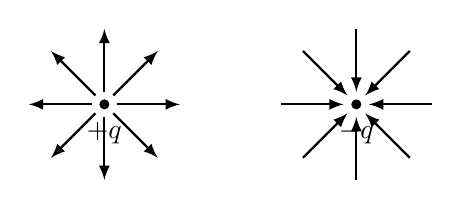
\begin{tikzpicture}[scale=0.8]
    % Поле положительного заряда
    \filldraw[black] (0,0) circle (2pt) node[below=3pt] {$+q$};
    \foreach \a in {0,45,90,135,180,225,270,315}
        \draw[->, >=latex, thick] (\a:0.2) -- (\a:1.2);
    
    % Поле отрицательного заряда
    \begin{scope}[xshift=4cm]
        \filldraw[black] (0,0) circle (2pt) node[below=3pt] {$-q$};
        \foreach \a in {0,45,90,135,180,225,270,315}
            \draw[<-, >=latex, thick] (\a:0.2) -- (\a:1.2);
    \end{scope}
\end{tikzpicture}
\end{center}

Свойства линий напряжённости:
\begin{enumerate}
    \item Линии начинаются на положительных зарядах (или в бесконечности) и заканчиваются на отрицательных (или в бесконечности).
    \item Линии электростатического поля не замкнуты и не пересекаются.
    \item Густота линий пропорциональна модулю напряженности поля.
\end{enumerate}

\subsubsection{Потенциал}

\textbf{Потенциал $\varphi$} --- скалярная энергетическая характеристика электрического поля. Если напряженность $\vec{E}$ описывает силовое воздействие, то потенциал характеризует энергетический запас системы «заряд--поле».

Потенциал численно равен потенциальной энергии, которой обладает единичный положительный пробный заряд $q_0$, помещенный в данную точку:
\[
    \varphi = \frac{W_p}{q_0}
\]
Так как работа консервативных сил поля равна изменению потенциальной энергии, взятому с обратным знаком ($A = -\Delta W_p$), при перемещении заряда из данной точки в бесконечность (где $W_{p\infty} = 0$), работа $A_{1 \to \infty}$ совпадает с начальной энергией. Отсюда вытекает второе определение:
\[
    \varphi = \frac{A_{1 \to \infty}}{q_0}
\]
В системе СИ потенциал измеряется в \textit{Вольтах} (1 В = 1 Дж / 1 Кл).

Рассчитаем потенциал поля, создаваемого точечным зарядом $q$. Сила Кулона $F = k \frac{qq_0}{r^2}$ является консервативной. Работа этой силы по перемещению заряда $q_0$ из точки на расстоянии $r$ в бесконечность:
\[
    A_{1 \to \infty} = \int_{r}^{\infty} F dr = \int_{r}^{\infty} k \frac{qq_0}{r^2} dr = kqq_0 \left[ -\frac{1}{r} \right]_{r}^{\infty} = \frac{kqq_0}{r}
\]
Подставляя эту работу в определение потенциала ($\varphi = A/q_0$), получаем формулу для \textbf{потенциала точечного заряда}:
\[
    \varphi = \frac{kq}{r}
\]

На практике физический смысл имеет не абсолютное значение $\varphi$, а его изменение. Работа по перемещению заряда между точками 1 и 2:
\[
    A_{1 \to 2} = W_{p1} - W_{p2} = q(\varphi_1 - \varphi_2) = qU
\]
Здесь $U = \varphi_1 - \varphi_2$ — напряжение, характеризующее работу поля на конкретном участке пути.

\subsubsection{Связь поля с потенциалом}

Свяжем силовую ($\vec{E}$) и энергетическую ($\varphi$) характеристики. Элементарная работа силы поля на малом перемещении $d\vec{l}$:
\[
    dA = \vec{F} \cdot d\vec{l} = q\vec{E} \cdot d\vec{l}
\]
С другой стороны, та же работа равна убыли потенциальной энергии: $dA = -dW_p = -q d\varphi$. Приравнивая выражения, получаем $\vec{E} \cdot d\vec{l} = -d\varphi$. В трехмерном пространстве эта связь выражается через оператор \textbf{градиента}:
\[
    \vec{E} = -\text{grad}\,\varphi = -\nabla\varphi = -\left( \frac{\partial\varphi}{\partial x}\vec{i} + \frac{\partial\varphi}{\partial y}\vec{j} + \frac{\partial\varphi}{\partial z}\vec{k}\right)
\]
Знак «минус» указывает на то, что вектор напряженности $\vec{E}$ всегда направлен в сторону \textit{убывания} потенциала.

\subsubsection{Поток вектора напряженности}

\textbf{Поток вектора напряженности $\Phi_E$} --- скалярная физическая величина, которая наглядно характеризует количество линий напряженности электрического поля, пронизывающих некоторую поверхность $S$.

Рассмотрим малую площадку $dS$. Вектор площади $d\vec{S}$ направлен по нормали к этой площадке. Элементарный поток определяется как скалярное произведение:
\[
    d\Phi_E = \vec{E} \cdot d\vec{S} = E \cdot dS \cdot \cos \alpha
\]
где $\alpha$ — угол между вектором $\vec{E}$ и нормалью $\vec{n}$ к площадке.

Чтобы найти полный поток через поверхность $S$, необходимо проинтегрировать элементарные потоки:
\[
    \Phi_E = \int_S \vec{E} \cdot d\vec{S}
\]

\subsection{Теорема Гаусса}

\subsubsection{Формулировка}

Теорема Гаусса связывает поток вектора напряженности через \textit{замкнутую} поверхность с суммарным зарядом внутри этой поверхности.

Поток вектора напряженности $\vec{E}$ через произвольную замкнутую поверхность $S$ в вакууме равен алгебраической сумме зарядов, находящихся внутри этой поверхности, деленной на электрическую постоянную $\varepsilon_0$:
\[
    \Phi_E = \oint_S \vec{E} \cdot d\vec{S} = \frac{1}{\varepsilon_0} \sum_{i=1}^n q_i
\]

Из теоремы следует:
\begin{enumerate}
    \item Поток не зависит от формы поверхности, а только от величины заряда внутри.
    \item Заряды, находящиеся \textit{вне} поверхности, вклада в суммарный поток не дают (сколько линий вошло, столько и вышло).
\end{enumerate}

Если заряд распределен по объему с плотностью $\rho = dq/dV$, то, используя теорему Остроградского-Гаусса, можно перейти от потока через поверхность к интегралу по объему:
\[
    \oint_S \vec{E} \cdot d\vec{S} = \int_V \text{div} \vec{E} \cdot dV = \int_V \frac{\rho}{\varepsilon_0} dV
\]
Отсюда вытекает локальная связь в каждой точке пространства:
\[
    \text{div} \vec{E} = \frac{\rho}{\varepsilon_0}
\]

\subsubsection{Физический смысл дивергенции}

\textbf{Дивергенция} --- скалярная функция векторного поля, которая характеризует плотность источников этого поля в данной точке. 

С помощью оператора набла ($\nabla$) дивергенция записывается как скалярное произведение оператора на вектор поля:
\[
    \text{div} \vec{E} = \nabla \cdot \vec{E} = \frac{\partial E_x}{\partial x} + \frac{\partial E_y}{\partial y} + \frac{\partial E_z}{\partial z}
\]

Дивергенция позволяет судить о наличии источников или стоков поля в конкретной области пространства:

\begin{itemize}
    \item $\text{div} \vec{E} > 0$ --- из данной точки «выходит» больше линий поля, чем входит. В этой области находится положительный заряд ($+\rho$).
    
    \item $\text{div} \vec{E} < 0$ --- в данную точку «входит» больше линий поля, чем выходит. В этой области находится отрицательный заряд ($-\rho$).
    
    \item $\text{div} \vec{E} = 0$ --- поток через малый объем равен нулю (сколько линий вошло, столько и вышло). В этой точке нет зарядов, либо они скомпенсированы.
\end{itemize}

\subsection{Электрический ток}

\subsubsection{Постоянный и переменный ток}

\textbf{Электрический ток} --- процесс направленного переноса электрического заряда. Для существования тока необходимы: наличие свободных носителей заряда и наличие электрического поля (разности потенциалов).

\begin{enumerate}
    \item У \textbf{постоянного тока} знач. и направление не изменяются со временем \textit{(аккумуляторы, гальванические элементы, солнечные батареи)}.
    \item \textbf{Переменный ток} периодич. изменяется по величине и направлению.
\end{enumerate}

\subsubsection{Характеристики тока}

\textbf{Сила тока $I$} --- скалярная величина, равная заряду, проходящему через поперечное сечение проводника в единицу времени:
\[
    I = \frac{dq}{dt}
\]
\textbf{Плотность тока $\vec{j}$} --- векторная величина, характеризующая распределение тока по сечению проводника:
\[
    \vec{j} = n q \vec{v}_{\text{ср}}
\]
Направлена в сторону движения положительных зарядов. Связь с силой тока:
\[ I = \int_S \vec{j} \cdot d\vec{S} \]

\subsubsection{Закон Ома в дифференциальной форме}

Закон Ома в дифференциальной форме описывает связь между плотностью тока и напряженностью электрического поля в \textit{каждой точке} проводника.
\[
    \vec{j} = \sigma \vec{E}
\]

Физический смысл:
\begin{itemize}
    \item Плотность тока в данной точке среды прямо пропорциональна напряженности электрического поля в этой же точке.
    \item Вектор $\vec{j}$ сонаправлен с вектором $\vec{E}$.
\end{itemize}

\subsubsection{Закон Ома в интегральной форме}

Эта форма закона применяется к конкретным участкам электрических цепей.

Если на участке действует только электростатическое поле, то разность потенциалов совпадает с напряжением ($U = \varphi_1 - \varphi_2$).
\[
    I = \frac{U}{R}
\]

\textbf{Неоднородным} называется участок, на котором действуют сторонние силы --- силы неэлектростатической природы: химические, магнитные и т.д.. Характеристикой таких сил является \textbf{ЭДС} ($\mathcal{E}$).

Полная напряженность поля на таком участке: $\vec{E}_{total} = \vec{E}_{coul} + \vec{E}_{ext}$.
Интегрируя закон Ома в дифференциальной форме вдоль участка цепи, получаем:
\[
    I = \frac{\varphi_1 - \varphi_2 + \mathcal{E}_{12}}{R + r},
\]
где:
\begin{itemize}
    \item $(\varphi_1 - \varphi_2)$ — работа кулоновских сил.
    \item $\mathcal{E}_{12}$ — работа сторонних сил.
\end{itemize}

Для цепи, представляющей собой замкнутый контур ($\varphi_1 = \varphi_2$):
\[
    I = \frac{\mathcal{E}}{R + r}
\]
где $R$ — внешнее сопротивление, $r$ — внутреннее сопротивление источника тока.

\begin{center}
\begin{tblr}{
    colspec = {X[1.2,l]X[2,l]},
    vlines, hlines,
    row{1} = {font=\bfseries, bg=gray!10},
    rowsep = 4pt
}
Параметр & Описание \\
Сопротивление $R$ & Характеризует противодействие проводника току: $R = \rho \frac{l}{S}$. Измеряется в Омах [Ом]. \\
Удельное сопротивление $\rho$ & Свойство материала: $\rho = \rho_0(1 + \alpha \Delta T)$. Измеряется в [Ом$\cdot$м]. \\
Проводимость $G$ & Величина, обратная сопротивлению: $G = \frac{1}{R}$. Характеризует способность участка цепи проводить ток. \\
Удельная проводимость $\sigma$ & Величина, обратная удельному сопротивлению: $\sigma = \frac{1}{\rho}$. Характеризует способность вещества проводить ток. \\
\end{tblr}
\end{center}

\subsubsection{Электроны в кабеле зарядки}

В USB-кабеле, изготовленном из меди, протекает постоянный электрический ток силой $I = 3{,}2$ А. 
Площадь поперечного сечения проводника составляет $S \approx 0{,}2 \, \text{мм}^2$.
Найти среднюю скорость $\langle v \rangle$ свободных электронов в проводнике:

\begin{center}
\begin{tikzpicture}[scale=1.2]
    % Проводник - толстые контуры для ч/б
    \draw[very thick] (0,0.5) -- (4,0.5);
    \draw[very thick] (0,-0.5) -- (4,-0.5);
    \draw[very thick] (0,0) ellipse (0.2 and 0.5);
    \draw[very thick] (4,0) ellipse (0.2 and 0.5);
    
    % Штриховка для обозначения сечения проводника
    \fill[pattern=north east lines, pattern color=black!40, opacity=0.7] 
          (4,0) ellipse (0.2 and 0.5);
    \node[below] at (4, -0.6) {$S$};
    
    % Электроны - заливка черным или штриховка
    \foreach \x in {1, 2, 3} {
        \foreach \y in {-0.2, 0.2} {
            \fill[pattern=crosshatch dots, pattern color=black!70] 
                  (\x + \y, \y) circle (0.1);
            \draw[->, thick, >=stealth] (\x + \y, \y) -- (\x + \y + 0.4, \y);
        }
    }
    
    % Ток - толстая стрелка
    \draw[->, ultra thick, >=stealth] (1.2, 0.8) -- (2.5, 0.8) 
          node[midway, above] {$I$};
\end{tikzpicture}
\end{center}

Сила тока $I$ — это заряд $\Delta q$, проходящий через поперечное сечение проводника за единицу времени $\Delta t$:
\[ I = \frac{\Delta q}{\Delta t} \]

Заряд $\Delta q$ можно выразить через общее количество частиц $N$:
\[ \Delta q = e \cdot N = e \cdot (n \cdot V) = e \cdot n \cdot (S \cdot \Delta l) \]
где $\Delta l = \langle v \rangle \cdot \Delta t$ — расстояние, которое проходят электроны за время $\Delta t$.

Подставим выражение для $\Delta q$ в формулу силы тока:
\[ I = \frac{e \cdot n \cdot S \cdot \langle v \rangle \cdot \Delta t}{\Delta t} = e \cdot n \cdot S \cdot \langle v \rangle \]

Отсюда выразим среднюю скорость электронов:
\[ \boxed{\langle v \rangle = \frac{I}{e \cdot n \cdot S}} \]

Концентрацию свободных электронов можно найти через плотность меди $\rho$, молярную массу $M$ и число Авогадро $N_A$, считая, что каждый атом меди даёт один свободный электрон:
\[ 
n = \frac{N}{V} = \frac{\nu N_A}{V} = \frac{\rho N_A}{M}\approx \frac{8{,}96\cdot10^3 \cdot 6{,}022\cdot10^{23}}{63{,}5\cdot10^{-3}} \approx 8{,}5\cdot10^{28}\ \text{м}^{-3}
\]

Подставим значения для медного провода:
\[ 
\langle v \rangle = \frac{3{,}2}{1{,}6 \cdot 10^{-19} \cdot 8{,}5 \cdot 10^{28} \cdot 0{,}2 \cdot 10^{-6}}\approx 1{,}17\ \text{мм/с} 
\]